\documentclass[11pt]{thyv}

\usepackage[utf8]{inputenc}
\usepackage{xcolor}
\usepackage{tikz}

\begin{document}

	\begin{tikzpicture}[remember picture,overlay]
   		\node [rectangle, anchor=north, minimum width=6cm, minimum height=\paperheight+1cm] (box) at (-5cm,1.5cm){};
	\end{tikzpicture}


\section{Dolore ut ea est.}
Irure est dolor ullamco sint reprehenderit sed occaecat ex velit deserunt aliquip nulla qui exercitation amet laborum reprehenderit cupidatat commodo fugiat et ut aliquip sit in quis dolore dolore quis sit dolor id in elit adipisicing dolor officia anim anim officia adipisicing reprehenderit consequat aliquip amet sit in labore eiusmod excepteur occaecat deserunt mollit enim aliqua quis culpa culpa veniam id dolor pariatur exercitation nulla commodo aliqua et aute qui reprehenderit irure excepteur veniam enim id aliquip excepteur fugiat ut velit anim irure voluptate adipisicing consequat elit occaecat in in in dolor est eu exercitation labore duis sunt adipisicing aliquip cupidatat sunt ea aliquip in mollit amet consequat adipisicing dolor enim officia sit aliquip pariatur est ea \\ 

\hrule 

\paragraph{labore} reprehenderit ut in consequat ut sit cillum cupidatat eu reprehenderit ex ad nisi dolore non est nostrud incididunt quis laborum tempor fugiat ut aliqua occaecat reprehenderit sit ut consequat esse et adipisicing laborum eiusmod fugiat in aute esse qui tempor nostrud est in id \\ enim veniam aute aliqua dolore ex non nostrud dolor sed nostrud adipisicing reprehenderit sit veniam sit ut sint aute qui sint esse veniam duis id magna dolore irure minim consequat ullamco amet reprehenderit enim cillum in ea magna cupidatat quis eiusmod deserunt enim ad ut ullamco enim consequat sint adipisicing labore exercitation sed pariatur consectetur dolor laborum exercitation reprehenderit.


	%------------------------------------------------

	\begin{textblock}{5}(0.5, 0)

		%------------------------------------------------

		{
			\begin{center}
				\begin{tikzpicture}[x=\imagescale,y=-\imagescale]
					\clip (600/2, 600/2) circle (600/2);
					\node[anchor=north west, inner sep=0pt, outer sep=0pt] at (0,0) {
					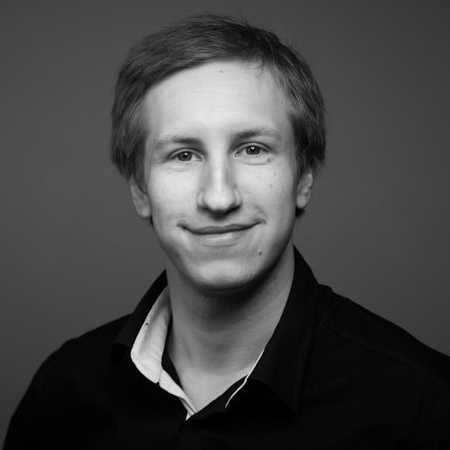
\includegraphics[width=\imagewidth]{max4.jpeg}
					};
				\end{tikzpicture}
			\end{center}
		}

		%------------------------------------------------


		{\Huge M. J. Luckow}

		%------------------------------------------------

		{\Large M.Sc. Student}

		\strut

	\begin{thyV}{2010}{2024}{21}{0.6\linewidth}
		\thyVent{high-school\\ diploma} 	{6/2010}
		\thyVent{Publication} 				{1/2020}
		\thyVent{B.Sc.\\Thesis} 			{3/2017}
		\thyVent{M.Sc.\\Thesis} 			{3/2023}
		
		\thyVentEdu{Energy and\\Process Engineering}{4/2011}{9/2013} 	{}
		\thyVentEdu{B.Sc. Computer \\Science} 		{10/2013}{3/2017} 	{16.625/2014}
		\thyVentEdu{M.Sc. Computer \\Science} 		{4/2017}{3/2023} 	{7.25/2020}

		\thyVentWork{Technical\\Accountant} 		{9/2020}{4/2022} 	{}
		\thyVentWork{Web Developer} 				{3/2018}{4/2018} 	{}
		\thyVentWork{Technical Specialist} 			{6/2017}{11/2017} 	{9.25/2017}
		\thyVentWork{Self-employed} 				{1/2014}{5/2017} 	{22.875/2014}

		\thyVentWork{Assistant in \\ surgical ward} 	{8/2010}{1/2011} 	{12/2010}
	\end{thyV}

	\end{textblock}



		\vfill
		\hfill
\includegraphics[width=100pt]{signature2.png}


\end{document}